\icode{N23L-MK-SI-L3-261001-002}
\nceeID[4]{2023山东}{6}
如图所示，电动公交车做匀减速直线运动进站，连续经过\(R\)、\(S\)、\(T\)三点，已知\(ST\)间的距离是\(RS\)间的两倍，\(RS\)段的平均速度是\qty{10}{m/s}，\(ST\)段的平均速度是\qty{5}{m/s}，则公交车经过\(T\)点时的瞬时速度是\paren[C]

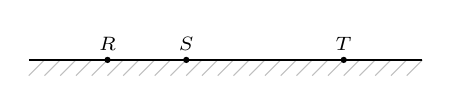
\begin{tikzpicture}[font=\scriptsize]
    \foreach \x in {-1,-.8,...,3.8}
        \draw[gray!50] (\x,-.2)--++(.2,.2);
    \draw[thick] (-1,0)--(4,0);
    \foreach \x/\str in{0/R,1/S,3/T}
        \fill (\x,0)node[above]{\(\str\)} circle(.04);
\end{tikzpicture}
\begin{choices}
    \item \qty{3}{m/s}
    \item \qty{2}{m/s}
    \item \qty{1}{m/s}
    \item \qty{0.5}{m/s}
\end{choices}
\begin{answer}
    C\qquad 提示：由两段位移与平均速度关系可知，若\(RS\)用时为\(\tau \)，则\(ST\)用时为\(4\tau\)

    \begin{tikzpicture}[>=stealth,font=\scriptsize]
        \draw[->,blue] (0,0)node[below left]{\(O\)}--(5,0)node[below]{\(t\)};
        \draw[->,blue] (0,0)--(0,4)node[right]{\(v\)/(\qty{}{m\cdot s^{-1}})};
        \draw[dashed,cyan] (0,3)node[blue,left]{10}--(.4,3)--(.4,0) (0,1.5)node[blue,left]{5}--(2.4,1.5)--(2.4,0)node[blue,below]{\(3\tau\)} (0,.3)--(4,.3)--(4,0)node[blue,below]{\(5\tau\)} (.8,2.7)--(.8,0)node[blue,below]{\(\tau\)};
        \draw[purple] (0,3.3)--(4,.3);
    \end{tikzpicture}
\end{answer}